\documentclass[tikz,border=8pt]{standalone}
% Shared look for every TikZ diagram. Load with \input{../../tools/tikz-style.tex}
\usepackage[T1]{fontenc}
\usepackage{lmodern}
\renewcommand{\sfdefault}{lmr}  % diagrams use the same serif as the text
\usetikzlibrary{arrows.meta, positioning, shapes.geometric, calc, fit, backgrounds}
\definecolor{cblue}{HTML}{4C78A8}
\definecolor{corange}{HTML}{F58518}
\definecolor{cgreen}{HTML}{54A24B}
\definecolor{cred}{HTML}{E45756}
\definecolor{cpurple}{HTML}{B279A2}
\definecolor{cgrey}{HTML}{6B6B6B}
\tikzset{
  every picture/.style={font=\sffamily, line width=1.2pt},
  box/.style={draw=#1, fill=#1!12, rounded corners=4pt, align=center, inner sep=7pt, minimum height=1.1cm},
  box/.default=cgrey,
  arrow/.style={-{Stealth[length=3mm]}, draw=cgrey, line width=1.4pt},
  title/.style={font=\sffamily\bfseries\Large},
  note/.style={font=\sffamily\small, text=cgrey, align=center},
}
\AtBeginDocument{\hyphenpenalty=10000 \exhyphenpenalty=10000}

% Two beams of the scan at pose A (2, 2, 0). The 90-degree beam reads 1.97 m: its endpoint (2, 3.97) is 0.03 m
% from the top wall. The forward beam reads 1.00 m (a person): its endpoint (3, 2) is 1.0 m from the nearest
% obstacle, the box corner (3.6, 1.2). The model looks only at each endpoint and that distance.
\begin{document}
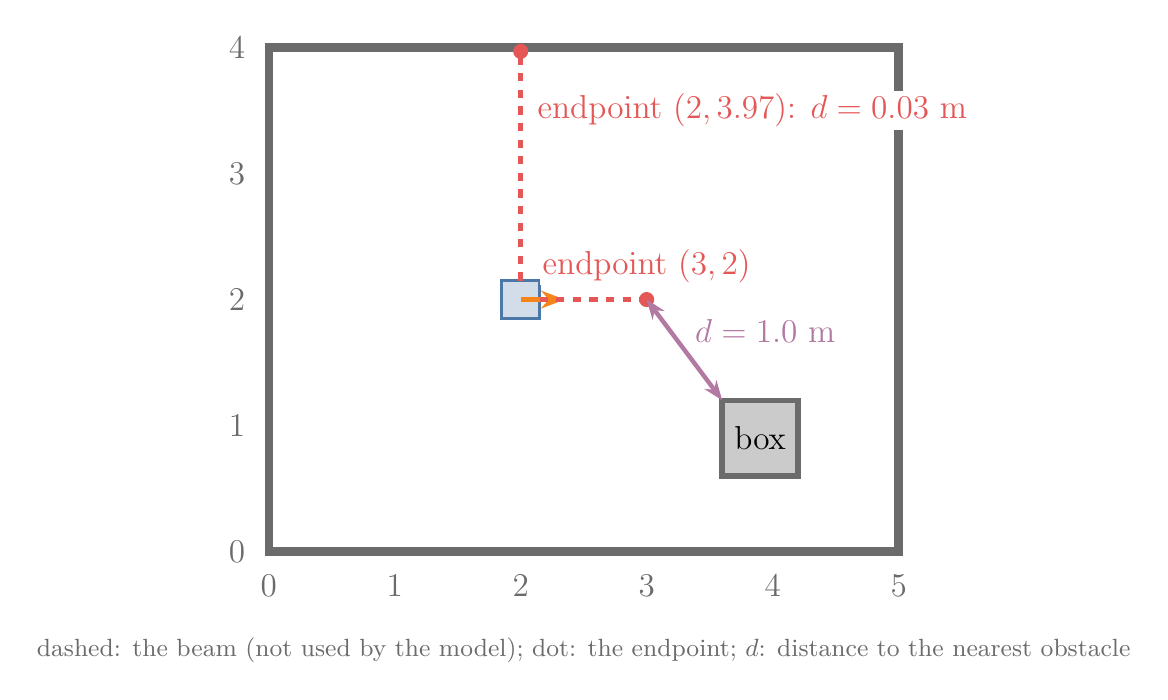
\begin{tikzpicture}[scale=1.6, every node/.append style={font=\large}]
  \draw[cgrey, line width=3pt] (0,0) rectangle (5,4);
  \draw[cgrey, fill=cgrey!35, line width=2pt] (3.6,0.6) rectangle (4.2,1.2);
  \node at (3.9,0.9) {box};
  \foreach \x in {0,1,...,5} \node[below, cgrey] at (\x,-0.1) {\x};
  \foreach \y in {0,1,...,4} \node[left, cgrey] at (-0.1,\y) {\y};
  \draw[cblue, fill=cblue!25] (1.85,1.85) rectangle (2.15,2.15);
  \draw[-{Stealth[length=3mm]}, corange, line width=2pt] (2,2) -- (2.35,2);
  % beam 90
  \draw[cred, line width=1.6pt, dashed] (2,2.15) -- (2,3.97);
  \fill[cred] (2,3.97) circle (0.06);
  \node[cred, right, fill=white, inner sep=1pt] at (2.1,3.5) {endpoint $(2, 3.97)$: $d = 0.03$ m};
  % beam 0
  \draw[cred, line width=1.6pt, dashed] (2.15,2) -- (3,2);
  \fill[cred] (3,2) circle (0.06);
  \draw[cpurple, line width=1.6pt, {Stealth[length=2.5mm]}-{Stealth[length=2.5mm]}] (3,2) -- (3.6,1.2);
  \node[cpurple, right, fill=white, inner sep=1pt] at (3.35,1.75) {$d = 1.0$ m};
  \node[cred, above, fill=white, inner sep=1pt] at (3.0,2.1) {endpoint $(3, 2)$};
  \node[note, anchor=north] at (2.5,-0.6) {dashed: the beam (not used by the model); dot: the endpoint; $d$: distance to the nearest obstacle};
\end{tikzpicture}
\end{document}
